\documentclass{article}

\usepackage{graphicx}
\usepackage{geometry}
\geometry{
  a4paper,
  total={170mm,257mm},
  left=20mm,
  top=20mm,
}
\usepackage{crimson}
\usepackage[T1]{fontenc}
\usepackage[round]{natbib}
\usepackage{nameref}
\usepackage{tikz}

\title{Evaluating isolation and contact tracing to control pandemic potential influenza outbreaks}
\author{Joshua W. Lambert}
\date{}

\begin{document}

\maketitle

\section*{Abstract}

\section*{Introduction}

Infectious disease outbreaks pose an everpresent public health threat. The COVID-19 pandemic caused over 7 million deaths \citep{whocovid-19dashboardCOVID19DeathsWHO}, while the 1918 influenza pandemic caused an estimated $\sim$50 million deaths \citep{johnsonUpdatingAccountsGlobal2002}. Less transmissible pathogens, such as Ebola, can cause sustained outbreaks leading to the excess death of thousands \citep{whoebolaresponseteamEbolaVirusDisease2014}. Thus, timely and accurate response is critical early in an outbreak when the pandemic or epidemic potential is still uncertain \citep{kucharskiControllingMinorOutbreaks2024}. An effective response requires understanding the efficacy and feasibility of intervention strategies across pathogens with varying epidemiological characteristics \citep{fraserFactorsThatMake2004}. \\

The likelihood of an outbreak being controlled, in other words going locally-extinct or -eliminated, is in part based on the epidemiological characteristics of the pathogen, and in part on the inventions implemented, both pharmaceutical and non-pharmaceutical. The primary epidemiological determinant for the spread of an infectious disease is the reproduction number ($R$), defined as the average number of secondary cases  per primary case. The higher the reproduction number the less likely a disease, without intervention, is to cease transmission in a population. If a pathogen is subcritical (i.e. $R < 1$) it will eventually stop spreading but can still cause transient outbreaks \citep{farringtonDistributionTimeExtinction1999}. Individual-level heterogeneity in transmission also influences the possibility of a pathogen going extinct from stochasticity in the transmission process \citep{lloyd-smithSuperspreadingEffectIndividual2005}. Higher individual-level variation for a given reproduction number leads to, on average, more outbreaks being controlled (however a small number of outbreaks may become large due to superspreading). In addition, the likelihood of containment is reduced --- assuming $R > 1$ --- if there are multiple introductions into a populations \citep{kucharskiEarlyDynamicsTransmission2020}. \\

A range of interventions can be deployed to reduce or prevent the transmission of infectious diseases, broadly classified into pharmaceutical and non-pharmaceutical interventions (NPIs). Early in an outbreak --- especially in the case of a novel pathogen --- NPIs are often the first line of defence, as pharmaceutical options may not yet be available. These interventions vary in scope and specificity, from targeted measures such as isolation and contact tracing, to broader actions like school closures, bans on gatherings, and regional or national lockdowns (Huag et al., 2020). The success of such interventions in containing an outbreak before it becomes sustained and widespread depends on several factors, including the type of intervention, the delay before implementation, and the intervention’s effectiveness (Longini et al., 2005). For highly transmissible pathogens (e.g. $R>3$) with short generation times (e.g. $<3$ days), swift and effective interventions are required to achieve containment. Pathogens that have a large proportion of onward transmission prior to symptom onset (latent period shorter than incubation period) or have asymptomatic (subclinical) cases are less easily controlled \citep{fraserFactorsThatMake2004}. \\

Contact tracing, the process of finding the contacts of infected individuals is an often used NPI to try and curtail the growth of an epidemic. It can involve forward contact tracing, whereby infected individuals are asked who they have been in contact with so their contacts can be followed-up and isolated or quarantined if needed; or backward contact tracing whereby infected individuals are asked who they have been in contact with prior to being infected to identify the source of infection and potentially forward trace from the source. Isolation and contact tracing is a targeted approach, like ring vaccination, that looks to prevent the onward transmission of an infectious disease by tackling infected individuals and their contacts \citep{kucharskiEffectivenessRingVaccination2016, ferrettiQuantifyingSARSCoV2Transmission2020, keelingEfficacyContactTracing2020, whittakerQuantifyingImpactBroadly2024}. Isolation or vaccination of traced individuals has proved widely effective in controlling different outbreaks with a variety of pathogens differing in their aetiological and epidemiological characteristics \citep{foegeSELECTIVEEPIDEMIOLOGICCONTROL1971, bellPublicHealthInterventions2004}. However, it's important to remember that it's not a panacea for all outbreak scenarios. In epidemics or pandemics where the proportion of cases or contacts missed is high, either because surveillance is patchy or because the number of contacts exceeds the capacity of the system, the efficacy of contact tracing to contain an outbreak diminishes, or at worst, fails completely \citep{dhillonWhenContactTracing2018, hellewellFeasibilityControllingCOVID192020}. \\

It has become widely accepted that influenza viruses cannot be controlled with isolation and contact tracing because the rate at which infected individuals become infectious and show symptoms is faster than the latency in the process of contacting contacts (Fraser et al., 2004; Klinkenberg et al., 2006). However, with the recent human infections of avian influenza (A/H5N1), mostly among poultry and cattle farmers (Garg et al., 2025) and the longer estimates of incubation period and serial interval (SI) from historical H5N1 data \citep{Ward2024.12.11.24318702} it may be that isolation and contact tracing is able to control influenza. The (antigenic) novelty of a pathogen introduced into a human population is a leading risk factor for causing a pandemic. Thus, influenza subtypes that have negligible levels of existing immunity in the population are probable epidemic and pandemic candidates. This is the case for H5N1 and H7N9 \citep{tannerPandemicPotentialAvian2015} and was the case when H1N1 caused an outbreak in 2009 \citep{fraserPandemicPotentialStrain2009}. Historically, avian influenza (H5N1 and H7N9) have had high severity (case fatality risk $\sim 35\%-55\%$), and therefore sustained transmission in a human population could have substantial mortality and morbidity implications \citep{tannerPandemicPotentialAvian2015}. \\

In this study we evaluate the effectiveness of controlling infectious disease outbreaks that exhibit influenza-like epidemiological characteristics using a mathematical model. In effect the ability to control an epidemic with isolation and contact tracing is a race between the identification and isolation of contacts and the spread of the infectious agent (Reyna-Lara et al., 2021). The dogma that influenza contagion outpaces our ability to trace and isolate in time, may not hold for all pathogen subtypes with new estimates of incubation period and serial interval (Ward et al., 2024). This study looks to define the speed and effectiveness of isolation under different response delays across epidemic scenarios to inform outbreak response; quantifying the impact of reducing the delay to isolation on outbreak containment and the utility of rapid testing.

\section*{Methods}

\subsection*{Branching process model with isolation}

To assess the efficacy of isolation and contact tracing to control an outbreak of pandemic-potential influenza we used an individual-level transmision model implemented in the R package \texttt{\{ringbp\}} \citep{hellewellRingbpSimulateEvaluate2025} (Figure \ref{fig:ringbp-model}). The epidemic simulation model uses a single-type branching process with a negative binomial offspring distribution to simulate the spread of a pathogen through a population (infinite population size, without depletion of susceptibility). The mean of the negative binomial offspring distribution is the basic reproduction number ($R$), and this distribution allows the model to be parameterised to capture overdispersion of transmission, in other words, some infectors are superspreaders and infect a disproportionate number of individuals \citep{lloyd-smithSuperspreadingEffectIndividual2005, kucharskiEarlyDynamicsTransmission2020}. \\

There are three categories for individuals in the simulation, with each having their own parameterisation for the negative binomial offspring distribution: 1) \textit{community} (i.e. general population), 2) \textit{isolated}, and 3) \textit{asymptomatic}. Each group have a distinct $R$ and dispersion ($k$) parameter due to the assumed differences in transmission dynamics between groups. \\

The time between an infector being infected and then infecting an infectee (i.e. generation time) is indirectly computed using the incubation period (which samples the symptom onset time from the exposure time of each case) and sampling from a skew-normal distribution \citep{azzaliniClassDistributionsWhich1985}. This controls the proportion of the infections that occur prior to, or after, the symptom onset of an infector. The symptom onset time is used as the location parameter ($\xi$) of the distribution, providing the point around which the distribution is dispersed. The scale parameter ($\omega$) is fixed at two, this parameter (with the shape parameter) defines the variance of the distribution. We select this value as to provides a realistic amount of variance when transforming onset time to exposure time (variance range for scenarios in this study: 1.5 - 3.2). The shape parameter ($\alpha$) defines the skewness of the distribution, whereby positive values cause right-skewed values distribution around the location $\xi$, and negative values have the opposite effect (as $\alpha \rightarrow \infty$, the skew-normal converges to a folded-normal distribution). In summary, for a given parameterisation of the skew-normal distribution given the time of symptom onset ($\xi$) and fixing $\omega$ and $\alpha$ we sample the time an infectee is exposed/infected by an infector. \\

The NPI implemented in the transmission model is an isolation of symptomatic cases and contact tracing (Figure \ref{fig:ringbp-model}). When a case is symptomatic they are isolated after a delay. The timing of isolation is drawn from the onset-to-isolation distribution (see \nameref{epiparameters} section for parameterisation). Any infection times that are sampled to occur after the isolated of an infector are remove, because isolation is assumed completely effective at preventing further transmission, reducing the number of secondary cases if the speed of isolation is quicker than some or all of the secondary infection times. In other words, once a case is isolated at time $t_{isolated}$, the probability of that case infecting anyone at $t > t_{isolated}$ is zero. Another way to interpret the model is that $R$ is composed of secondary infections before isolation ($R_{pre}$) and secondary infections after an assumed isolation time ($R_{isolated}$). Symptomatic individuals that are traced are isolated either when 1) the onset-to-isolation delay after symptom onset, or 2) the infector is isolated. The isolation of the infectee is whatever occurs first of these two events.  \\

There are several mechanisms where isolation and contact tracing are imperfect at reducing onward disease transmission. The proportion of contacts missed by contact tracing is defined by the proportion of ascertainment and can range between zero, that is nobody is traced, to one, every case is traced. Symptomatic cases that have been missed when contact tracing their infectors are isolated at the onset-to-isolation delay after their symptom onset time. Additionally, contact tracing misses infections by an asymptomatic infector. In this event the infectees are missed by contact tracing owing to the infector not being known to the response system. \\

\begin{figure}[ht]
\centering
{\sffamily
  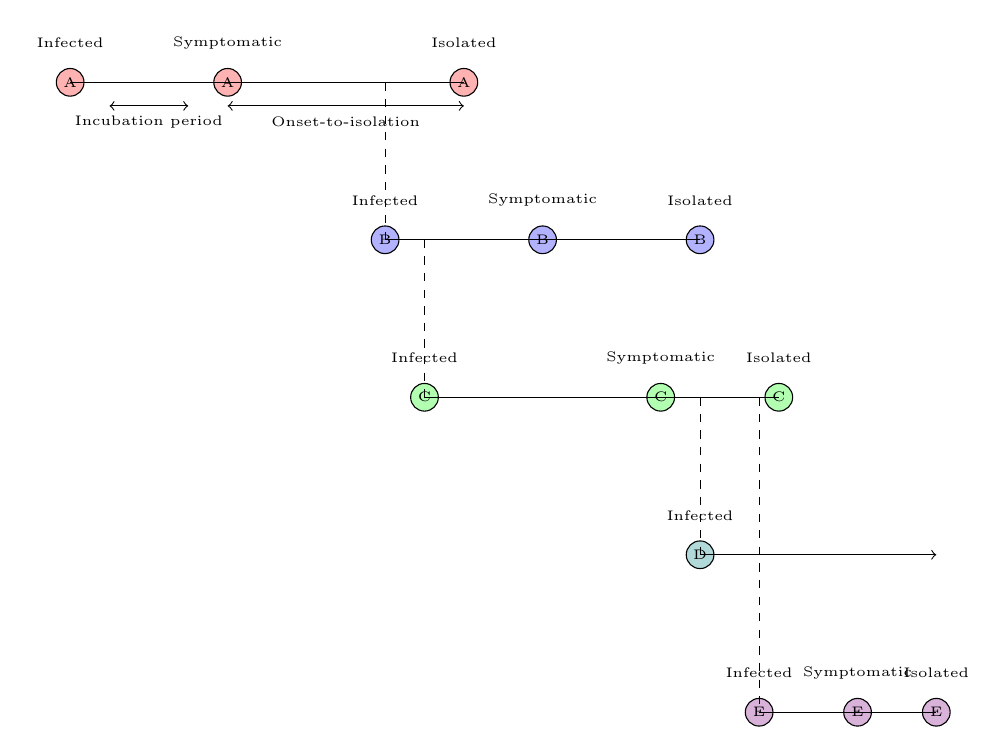
\begin{tikzpicture}[every node/.style={font=\tiny}]
  % Labels above the A row
  \node at (0,0.5) {Infected};
  \node at (2,0.5) {Symptomatic};
  \node at (5,0.5) {Isolated};

  % Top row: A circles with red background
  \fill[red!30] (0,0) circle (5pt);
  \draw (0,0) circle (5pt);
  \node at (0,0) {A};

  \fill[red!30] (2,0) circle (5pt);
  \draw (2,0) circle (5pt);
  \node at (2,0) {A};

  \fill[red!30] (5,0) circle (5pt);
  \draw (5,0) circle (5pt);
  \node at (5,0) {A};

  % Horizontal line between A circles
  \draw (0,0) -- (2,0);
  \draw (2,0) -- (5,0);

  % Individual A delays
  \draw[<->] (0.5,-0.3) -- (1.5,-0.3);
  \node at (1,-0.5) {Incubation period};
  \draw[<->] (2,-0.3) -- (5,-0.3);
  \node at (3.5,-0.5) {Onset-to-isolation};

  % Labels above the B row
  \node at (4,-1.5) {Infected};
  \node at (6,-1.5) {Symptomatic};
  \node at (8,-1.5) {Isolated};

  % Middle row: B circles with blue background
  \fill[blue!30] (4,-2) circle (5pt);
  \draw (4,-2) circle (5pt);
  \node at (4,-2) {B};

  \fill[blue!30] (6,-2) circle (5pt);
  \draw (6,-2) circle (5pt);
  \node at (6,-2) {B};

  \fill[blue!30] (8,-2) circle (5pt);
  \draw (8,-2) circle (5pt);
  \node at (8,-2) {B};

  % Horizontal line between B circles
  \draw (4,-2) -- (6,-2);
  \draw (6,-2) -- (8,-2);

  % Labels above the C row
  \node at (4.5,-3.5) {Infected};
  \node at (7.5,-3.5) {Symptomatic};
  \node at (9,-3.5) {Isolated};

  % Bottom row: C circles with green background
  \fill[green!30] (4.5,-4) circle (5pt);
  \draw (4.5,-4) circle (5pt);
  \node at (4.5,-4) {C};

  \fill[green!30] (7.5,-4) circle (5pt);
  \draw (7.5,-4) circle (5pt);
  \node at (7.5,-4) {C};

  \fill[green!30] (9,-4) circle (5pt);
  \draw (9,-4) circle (5pt);
  \node at (9,-4) {C};

  % Horizontal line between C circles
  \draw (4.5,-4) -- (7.5,-4);
  \draw (7.5,-4) -- (9,-4);

  % Labels above the D row
  \node at (8,-5.5) {Infected};

  % Individual C circles with green background
  \fill[teal!30] (8,-6) circle (5pt);
  \draw (8,-6) circle (5pt);
  \node at (8,-6) {D};

  % arrow for asymptomatic D individual
  \draw[->] (8,-6) -- (11,-6); % arrow for asymptomatic

  % Labels above the C row
  \node at (8.75,-7.5) {Infected};
  \node at (10,-7.5) {Symptomatic};
  \node at (11,-7.5) {Isolated};

  % E individual
  \fill[violet!30] (8.75,-8) circle (5pt);
  \draw (8.75,-8) circle (5pt);
  \node at (8.75,-8) {E};

  \fill[violet!30] (10,-8) circle (5pt);
  \draw (10,-8) circle (5pt);
  \node at (10,-8) {E};

  \fill[violet!30] (11,-8) circle (5pt);
  \draw (11,-8) circle (5pt);
  \node at (11,-8) {E};

  % Horizontal line between E circles
  \draw (8.75,-8) -- (10,-8);
  \draw (10,-8) -- (11,-8);

  % Vertical dashed lines
  \draw[dashed] (4,0) -- (4,-2);   % A to B
  \draw[dashed] (4.5,-2) -- (4.5,-4);  % B to C
  \draw[dashed] (8,-4) -- (8,-6);  % C to D
  \draw[dashed] (8.75,-4) -- (8.75,-8);  % C to E

  \end{tikzpicture}
}
\caption{A schematic of the branching process model with isolation.}
\label{fig:ringbp-model}
\end{figure}

\subsection*{Defining outbreak control}

We use the same definition for outbreak control as \cite{hellewellFeasibilityControllingCOVID192020}: no new cases between 12 and 16 weeks after the start of an outbreak. The rationale for this criteria is that some outbreaks that do not take off and become large may still have a few cases for the first few weeks of an outbreak, therefore the window for control needs to be enough time after the seeding of an outbreak to be sure it is extinct. \\

There is also a maximum number of cases in simulation model, that when reached is judged to have reached a large epidemic and not controllable with 12-16 weeks. We set this limit to 500 cases. This number needs to be larger than the expected cluster size from an subcritical outbreak produce by chance (i.e. larger than $N_i / (1 - R)$, where $N_i$ is the number of initial cases and $R$ is the reproduction number).

\subsection*{Pathogen epidemiological parameters} \label{epiparameters}

In this study we evaluate the feasibility of controlling outbreaks of selected influenza subtypes that have previous caused sporadic human-to-human outbreaks with pandemic potential. We include A/H5N1, A/H1N1, and A/H7N9. These have caused outbreaks of various size and severity over the past 100 years. H5N1 has caused small outbreaks ($<$ 10 cases) of human-to-human transmission \citep{yangDetectingHumanhumanTransmission2007a, aditamaAvianInfluenzaH5N12012a}. H1N1 is now an endemic seasonal influenza with substantial population immunity, but a novel strain, H1N1pdm09, emerged in 2009 and caused a pandemic outbreak \citep{fraserPandemicPotentialStrain2009, lesslerOutbreak2009Pandemic2009}. \\

We extracted incubation periods from the epidemiological literature that have been previously estimated for the chosen Influenza subtypes. All incubation periods were found to be well described by a Weibull distribution, \cite{nishiuraEstimationIncubationPeriod2011} report the best fitting Weibull shape and scale parameters for H1N1 to be 1.77 and 1.86, respectively (Figure \ref{fig:incub}). \cite{cowlingComparativeEpidemiologyHuman2013} report the incubation period for H5N1 and H7N9, both Weibull distributed. For H5N1 the Weibull distribution has a mean of 3.3 days and standard deviation (SD) of 1.5 days, for H7N9 the Weibull distribution has a mean of 3.1 days and SD 1.4 days \citep{cowlingComparativeEpidemiologyHuman2013} (Figure \ref{fig:incub}). \\

The reproduction number ($R$) use to simulate transmission for each influenza subtype was 1.1, 1.5, 2.5 and 3.5. We chose these values and they represent either similar values to previously estimated $R$ values for influenza outbreaks \citep{fergusonStrategiesMitigatingInfluenza2006}, including H1N1 \citep{fraserPandemicPotentialStrain2009, lesslerOutbreak2009Pandemic2009}, or they represent an inflated values of current estimates of H5N1 and H7N9 subtypes to evaluate the effectiveness of isolation and contact tracing in the event that pathogen evolution (e.g. genetic reassortment (Peacock et al., 2025) or mutations in receptor binding preference (Lin et al., 2024)) enhances the human-to-human transmissibility of these pathogens. Current estimates for H5N1 and H7N9 subtypes are below unity (i.e. $R < 1$) (\citealt{tannerPandemicPotentialAvian2015}; \citealt{Ward2024.12.11.24318702}, but see \citealt{yangDetectingHumanhumanTransmission2007a} for a H5N1 $R$ estimate above 1) so transmission is expected to stop without intervention; with most outbreaks being small except in rare instances of superspreading events. Therefore evaluating isolation and contact tracing requires simulating outbreaks that have pandemic potential with exponential spread in the absence of control measures.

\begin{figure}[ht]
\centering
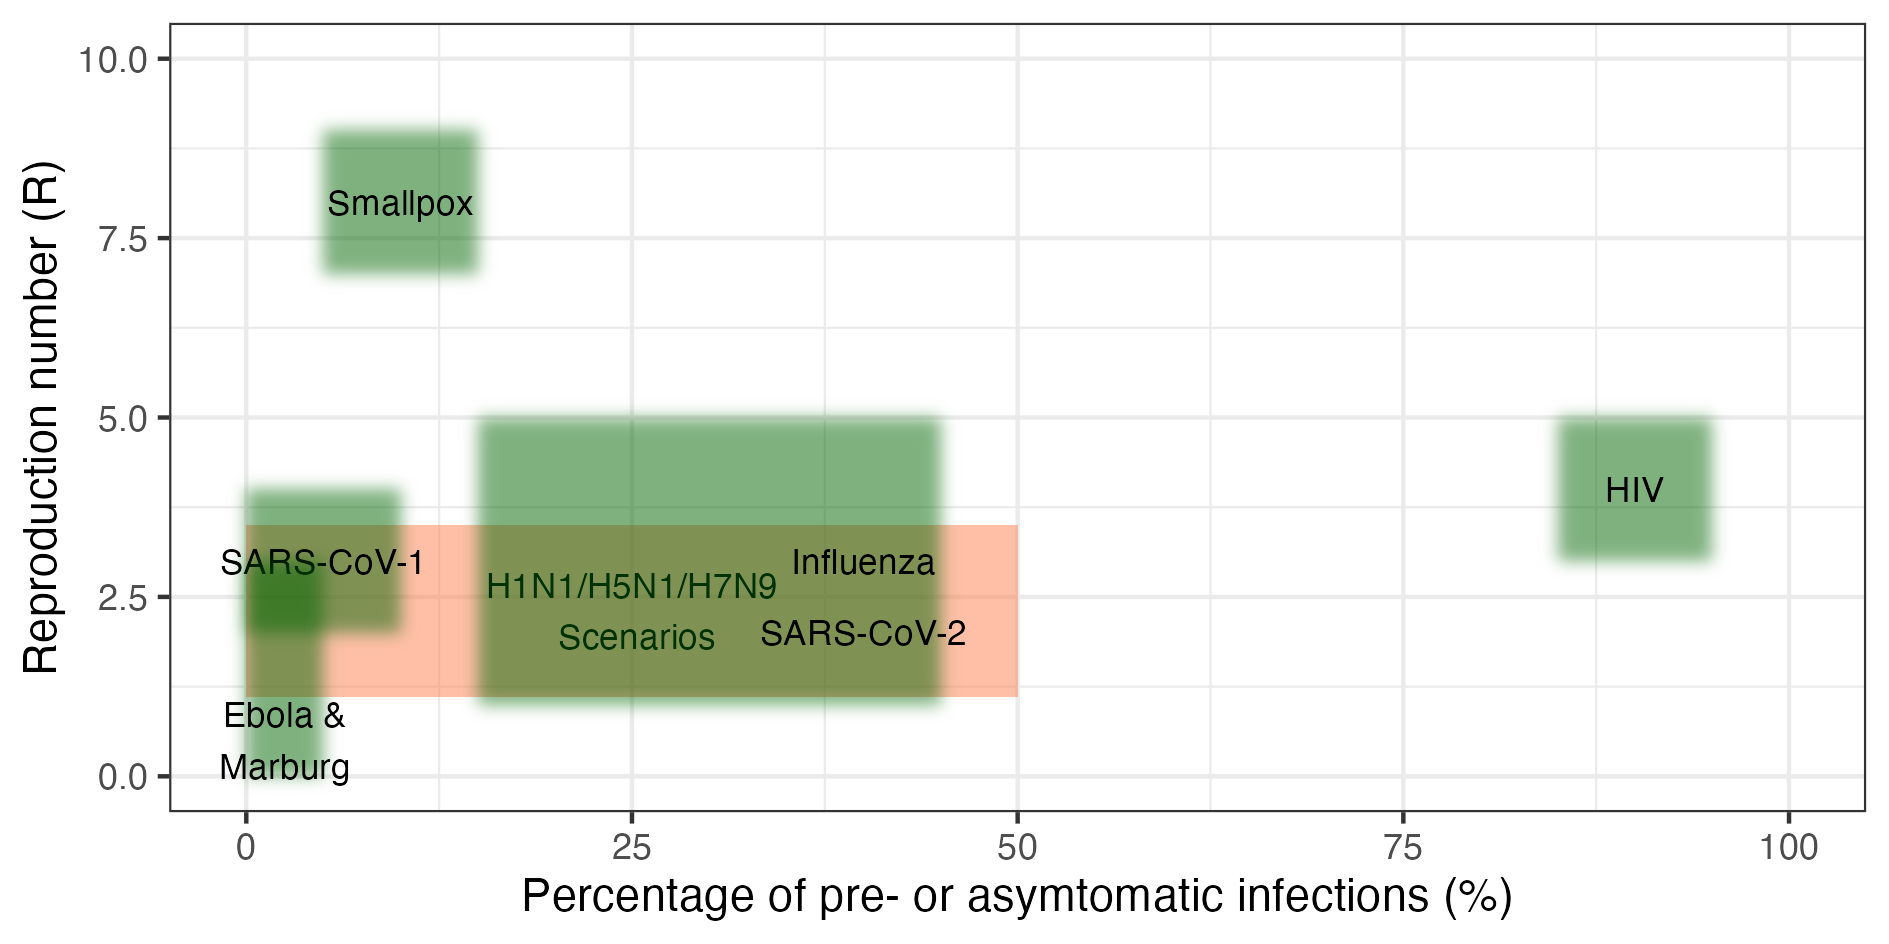
\includegraphics[width=\textwidth]{../plots/patho_param_space.png}
\caption{The pathogen characteristics, in terms of tranmissibility ($R$) and proportion of disease transmission that occurs before the onset of symptoms (including cases that are entirely asymptomatic). The figure includes: Influenza, SARS-CoV-1, SARS-CoV-2, Smallpox, Ebola, Marburg, and HIV shown by green shaded areas. The size of the shaded area reflects the differences in pathogen characteristics, both between variants and outbreaks, the blurred edges reflects uncertainty in parameter estimates. The parameter space of transmissibility and pre- and asymptomatic transmission explored in this paper is shown in the orange box.}
\label{fig:patho-param-space}
\end{figure}

\begin{figure}[ht]
\centering
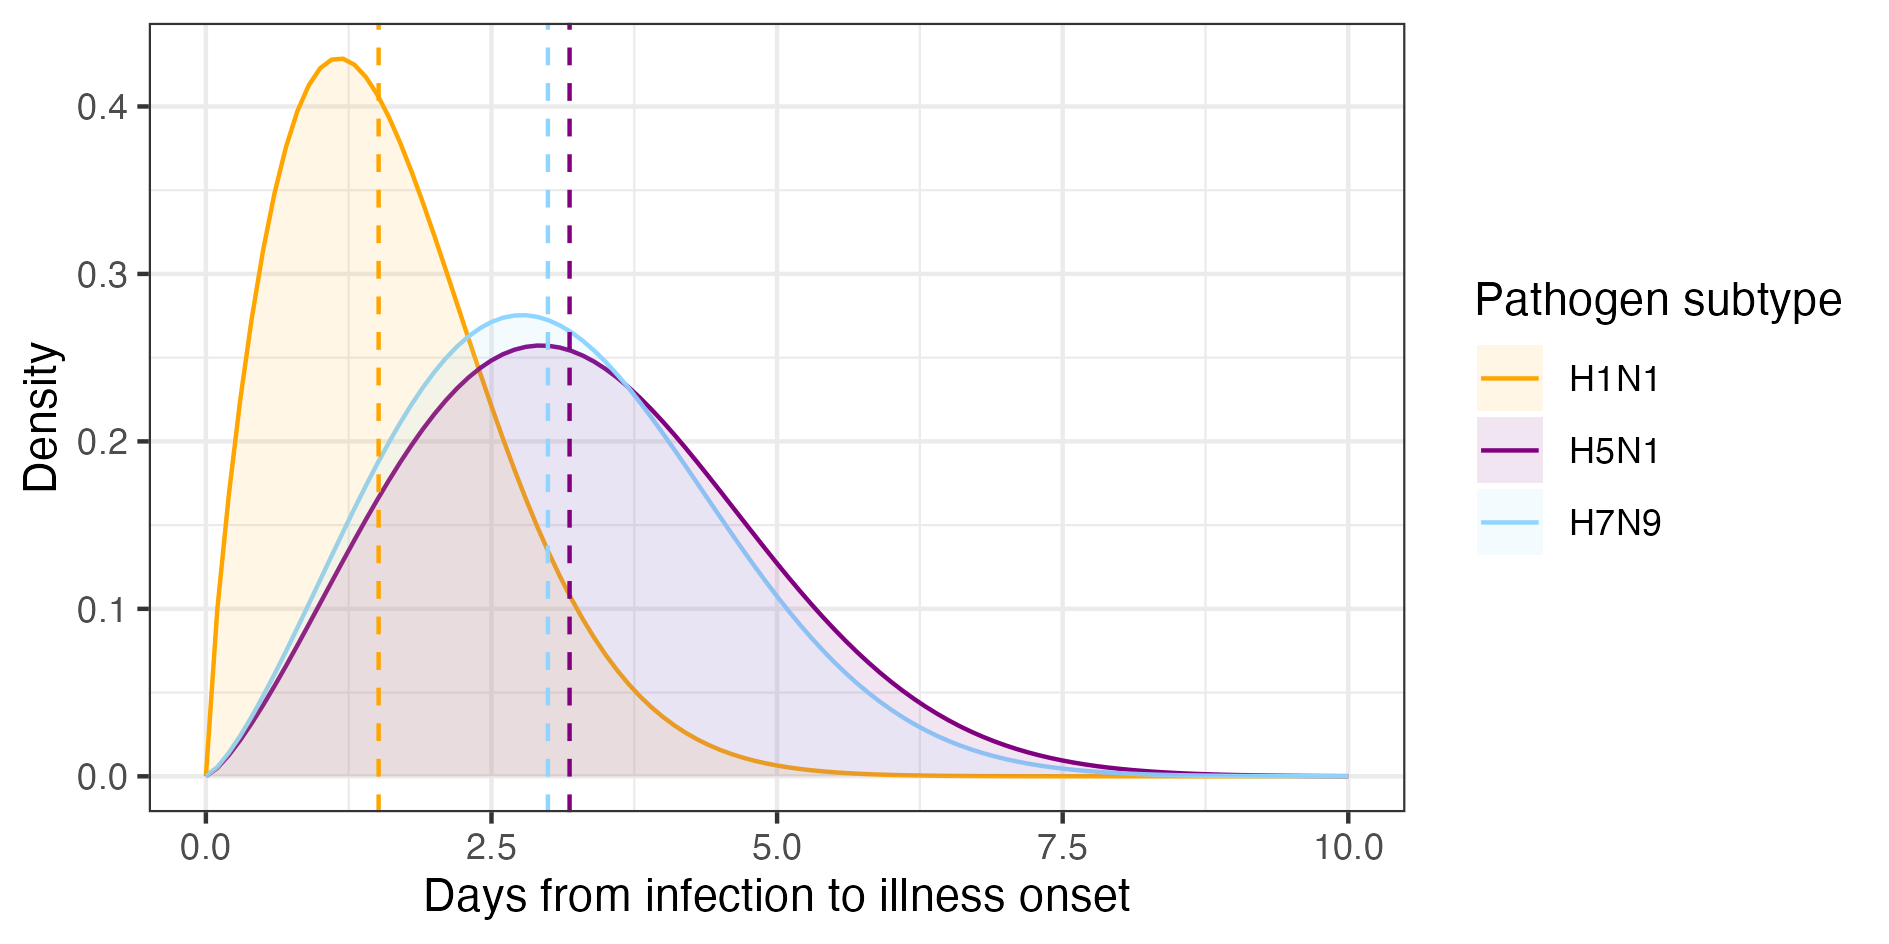
\includegraphics[width=\textwidth]{../plots/incubation_period.png}
\caption{Incubation period for the Influenza subtypes: H1N1, H5N1 and H7N9.}
\label{fig:incub}
\end{figure}

\clearpage

\subsection*{Simulation scenarios}

To assess under what scenarios pandemic-potential influenza outbreaks could be contained with the use of isolation and contact tracing we set up a simulation experiment. We defined a parameter space to explore across a variety of epidemiological characteristics (as defined in \nameref{epiparameters} section), contact tracing effectiveness, proportion of aysmptomatic cases and presymptomatic transmissin, and number of initial cases. \\

The ability to contain an outbreak by isolating infected individuals is highly contingent on the response time, or delay, between individuals becoming symptomatic, getting tested, the test results being returned and going into isolation. The probability that this series of steps will take an given amount of time is encapsulated in the onset-to-isolation delay distribution, i.e. onset-to-isolation distribution determines the time between a case developing symptoms and then becoming isolated. Here we define the onset-to-isolation as a response time as it is determined by the time delay between an individual responding to symptoms by getting tested and the turn around time for the tests to be analysed and the result returned. We view the onset-to-isolation as a feature of the public health outbreak response rather than an epidemiological characteristic of a disease. As such it is possible for pandemic response to adapt their response time to meet the needs of an outbreak. \\

We assume that an isolated case cannot transmit, so isolation is assumed to be 100\% effective once enacted ($R_{isolated} = 0$). The onset-to-isolation delay is parameterised with three scenarios: a fast response, based on the SARS in Hong Kong (Donnelly et al. 2003) and a slower response based on COVID-19 in Wuhan, China (Li et al. 2020) (Figure \ref{fig:onset-to-isolation}). Both the fast and slow onset-to-isolation are parameterised as Weibull distributions, the SARS-like distribution has shape ($\lambda$) 1.65 and scale ($k$) 4.29 (mean = 3.83 days, SD = 2.38 days), the COVID-like distribution has shape = 2.31 and scale = 9.48 (mean = 8.40, SD = 3.87 days) (Figure \ref{fig:onset-to-isolation}). These two empirically informed delay distributions provide a guide to possible response times in the case of an influenza outbreak and will enable us to evaluate if such delays are too long to contain a disease that can transmit rapidly such as influenza. We also include a third onset-to-isolation scenario based on the case where lateral flow rapid tests (LFTs) are provided to all individuals in the susceptible population and these people are freely able to self-test if they suspect they are symptomatic. We parameterise this as an exponential distribution, with rate ($\lambda$) 0.5, where most individuals will self-test very shortly after they become symptomatic (approximately 40\% of cases will self-test within the first day of sympmtom onset), with a few people waiting a 2 or more days before testing (approximately 3\% take longer than one week to take a self-test). \\

\begin{figure}[ht]
\centering
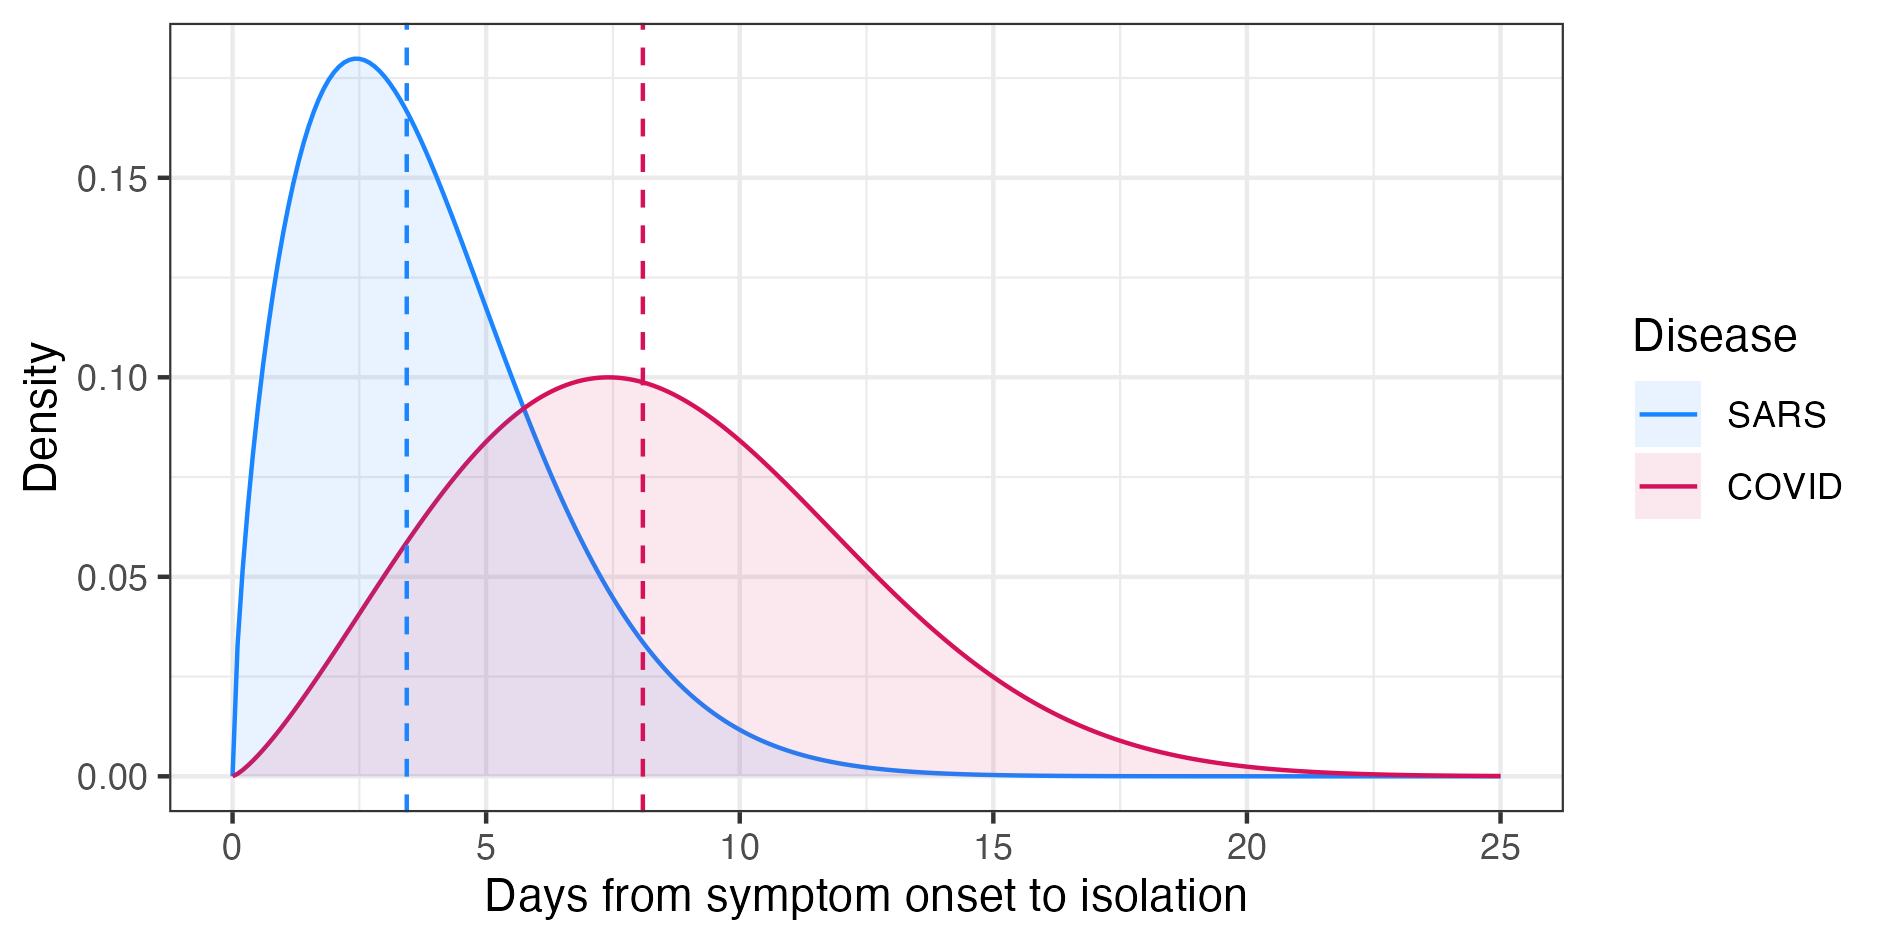
\includegraphics[width=\textwidth]{../plots/onset_to_isolation.png}
\caption{Three assumed onset-to-isolation delays used in the simuluation experiment. The \textit{Fast} scenario is based on the onset-to-isolation for SARS-CoV-1 response in Hong Kong (Donnelly et al. 2003), the median onset-to-isolation time is 3.4 days (blue dashed line). The \textit{Slow} scenario is based on the onset-to-isolation for the SARS-CoV-2 response in Wuhan, China (Li et al., 2020), the median onset-to-isolatiojn is 8.1 days (red dashed line). The lateral flow test (LFT) scenario is an assumed distributed for rapid self-administered home testing upon isolation, the median delay from symptom onset to isolation in this scenario is 1.4 days.}
\label{fig:onset-to-isolation}
\end{figure}

\clearpage

We define the proportion of pre-symptomatic transmission ($\theta$) follwowing the approach of \cite{hellewellFeasibilityControllingCOVID192020} by parameterising a skew-normal distribution to sample the infection times using the incubation period and a shape parameter ($\alpha$). The shape parameter controls the proportion of pre-symptomatic transmission by modulating the proportion of tranmission times that are less than the incubation time (Figure \ref{fig:prop-presym-trans}). We parameterise the skew-normal with three proportion of presymptomatic transmission scenarios: <1\%, 15\%, 30\%, these correspond to $\alpha$ values of 30, 1.95 and 0.7, respectively (Figure \ref{fig:prop-presym-trans}). Therefore, in all scenarios most transmission occurs after symptom onset, but due to isolation only impacting symptomatic individuals the greater proportion of transmission that occurs before symptom onset, the less effective contact tracing is hypothesied to be. \\

The proportion of pandemic-potential influenza infections that are asymptomatic varies for past outbreaks. There is evidence from past outbreaks of H1N1 and ??? that some laboratory (polymerase chain reaction) positive cases showed no symptoms or symptoms too mild to be considered influenza-like illness \citep{lesslerOutbreak2009Pandemic2009}. Here we assume that asymptomatic cases occur and can infect others, but are uncommon and that the majority of cases will develop symptoms during their infectious period.  We ran three scenarios, one with zero asymptomatic tranmission, another with 10\% of cases being asymptomatic and the most extreme scenario where 30\% of cases never develop symptoms and thus are not isolated and secondary cases are missed by contact tracing. \\

\begin{figure}[ht]
\centering
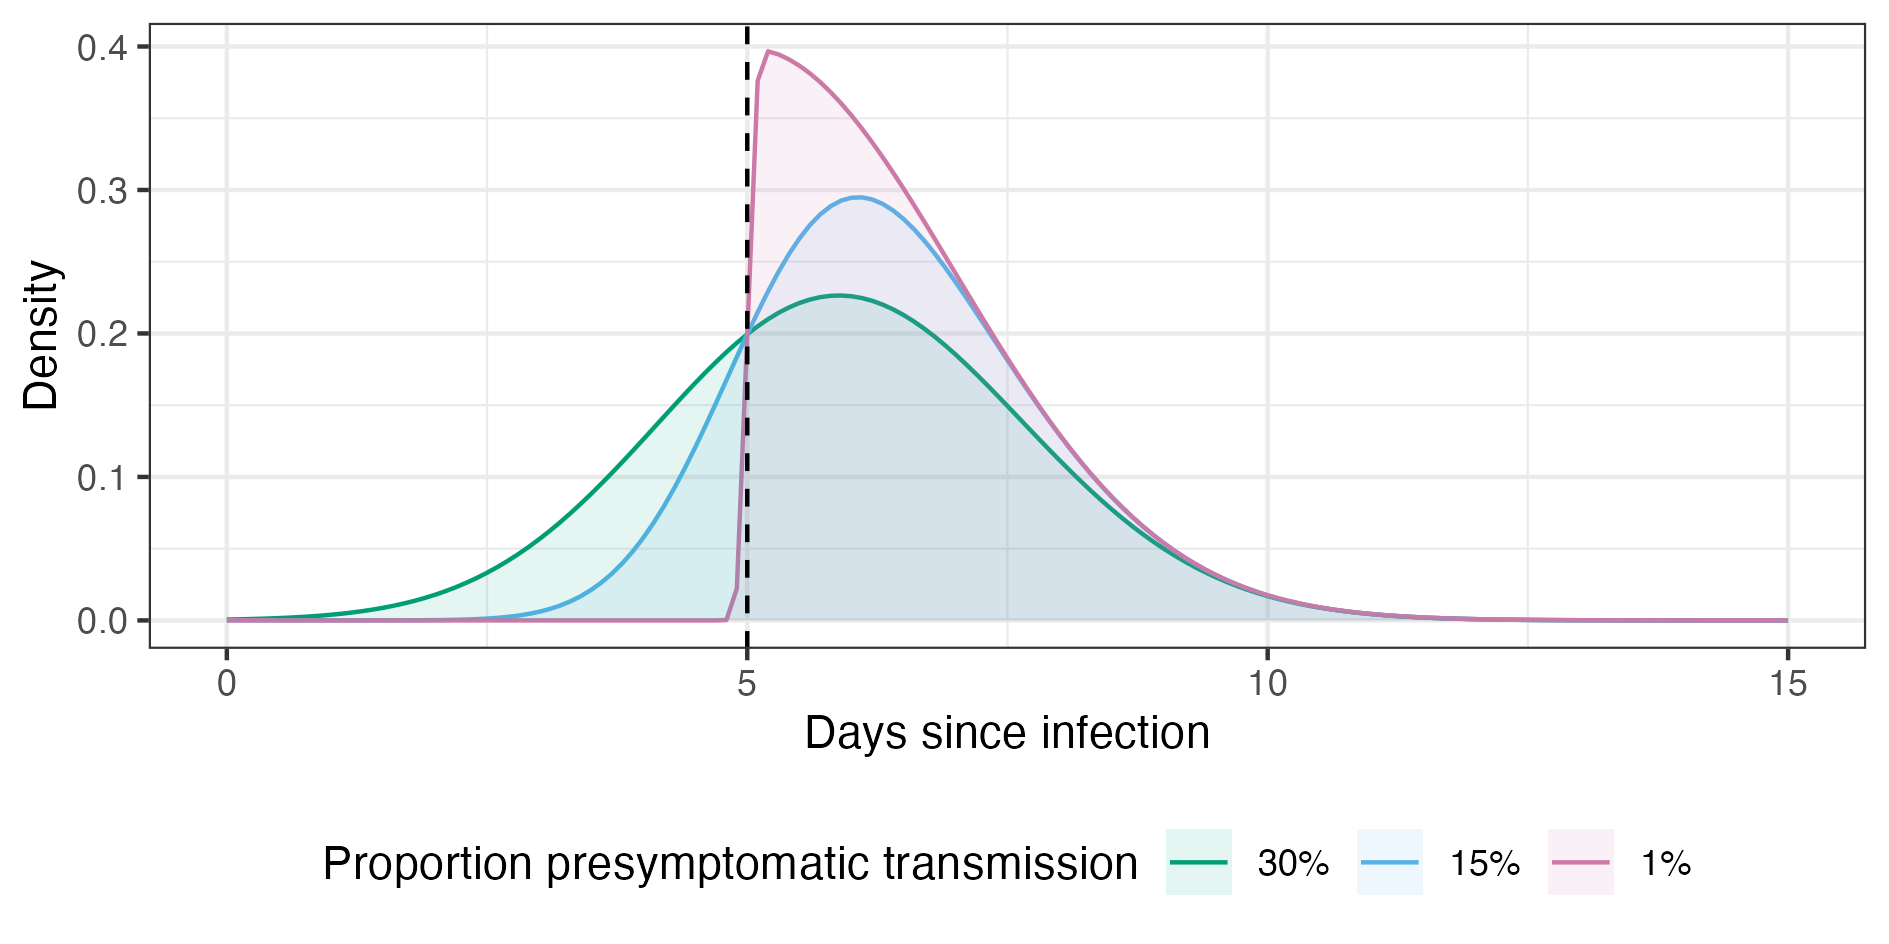
\includegraphics[width=\textwidth]{../plots/prop_presymptomatic_transmission.png}
\caption{Proportion of presymptomatic transmission determined by the incubation period, here assumed to be 5 days (dashed vertical line), controlled by a skew-normal distribution.}
\label{fig:prop-presym-trans}
\end{figure}

\clearpage

We simulated scenarios with either 5, 20 or 40 initial cases. This is to test whether contact tracing can contain outbreaks that may have already accumulated cases before contact tracing is started, or represents importation of multiple cases in a single event, such as a flight with multiple infectors (Khanh et al. 2020). \\

The proportion of ascertainment is varied between 0 and 1, at intervals of 0.2, to test at what proportion of missed cases would lead to outbreaks becoming uncontrolled epidemics. \\

Some parameters we fixed across all simulations. The dispersion parameter for the negative binomial offspring distribution was fixed at 1 for isolated cases, 0.16 for subclinical and community cases. For computational efficiency we capped the maximum number of days the simulation could run for to 365. This is substantially longer than the 12-16 week window for evaluating outbreak control so does not influence the results. Additionally, we limit simulations to 500 cases. This is an arbitrary threshold we judge to be large epidemic that is not controllable. \\

\section*{Results}

The incubation period for H1N1 is noticable shorter than the other two subtypes (H5N1 and H7N9), which are similar, with H5N1 having a slightly longer median (Figure \ref{fig:incub}). \\

Predictably, the ability to control an influenza epidemic is highly dependent on the reproduction number. A higher outbreak reproduction number results in a smaller percentage of outbreaks controlled at a given percentage of control effectiveness. (Figure \ref{fig:prop-outbreak-control-R}). There is a substantial difference between outbreaks with a $R$ slightly above unity ($R = 1.1$) which were controlled at a low levels ($\geq 20\%$) of isolation and contact tracing for all three influenza subtypes (Figure \ref{fig:prop-outbreak-control-R}). As $R$ increases to 1.5 there is a dramatic decline in the ability to control the epidemic without isolation of traced contacts (i.e. 0\% control effectiveness), however, outbreaks with $R = 1.5$ are mostly contained once control effectiveness exceeds 50\% (Figure \ref{fig:prop-outbreak-control-R}. Once the reproduction number is at 2.5 or 3.5, an outbreak is only controlled in at least 50\% of scenarios with isolation and contact tracing at greater than 60\% (Figure \ref{fig:prop-outbreak-control-R}). \\

The incubation period influences the efficacy of isolating and tracing. This effect is most pronounced when the percentage of outbreaks controlled is greater than 0\% and less than 100\% (i.e. not at the boundary) (Figure \ref{fig:prop-outbreak-control-R}). The shortest incubation period, H1N1, predominantly the least controllable for a given reproduction number, showing that infections that are symptomatic shortly after infection limit our ability to effectively tracing and isolate their potential infectees in time to prevent disease transmission. The difficulty to control an pandemic outbreak with a short incubation period is shown by the $\sim 40\%$ of simulated H1N1 outbreaks with 100\% control effectiveness that were not contained when $R = 3.5$, while longer incubation period outbreaks have $>80\%$ controlled when 100\% of contacts are traced and isolated (Figure \ref{fig:prop-outbreak-control-R}). Overall, both the transmissibility and incubation period impact the feasibility to control an outbreak. \\

The variance between the influenza subtypes at each percentage of contacts traced and isolated varies (i.e. difference between circle, triangle and square points at each contacts traced \% in Figure \ref{fig:prop-outbreak-control-R}). This variance is greatest at intermediate (20\% - 80\%) contact tracing effectiveness and intermediate values of $R$ (1.5 and 2.5) (Figure \ref{fig:prop-outbreak-control-R}). This could indicate a substantive role for incubation period durartion in the control of disease transmission. However, this variance in proportion of outbreaks controlled between pathogen subtypes does not show a strong pattern across all scenarios simulated (Figure \ref{fig:prop-outbreak-control-var-R}). There is a weak pattern of increased variance in controllability between subtypes at intermediate values of $R$, overall it seems that incubation period causes differences in control-by-isolation effectivness when not at the boundary of epidemic controllability. In other words, differences between influenza subtypes arise when not in a situation of high transmissibility and low contact tracing effectivness that cannot contain any outbreaks, nor low transmissibility and high contact tracing effectivenss easily contain all outbreaks (Figure \ref{fig:prop-outbreak-control-var-R}). \\

\begin{figure}[ht]
\centering
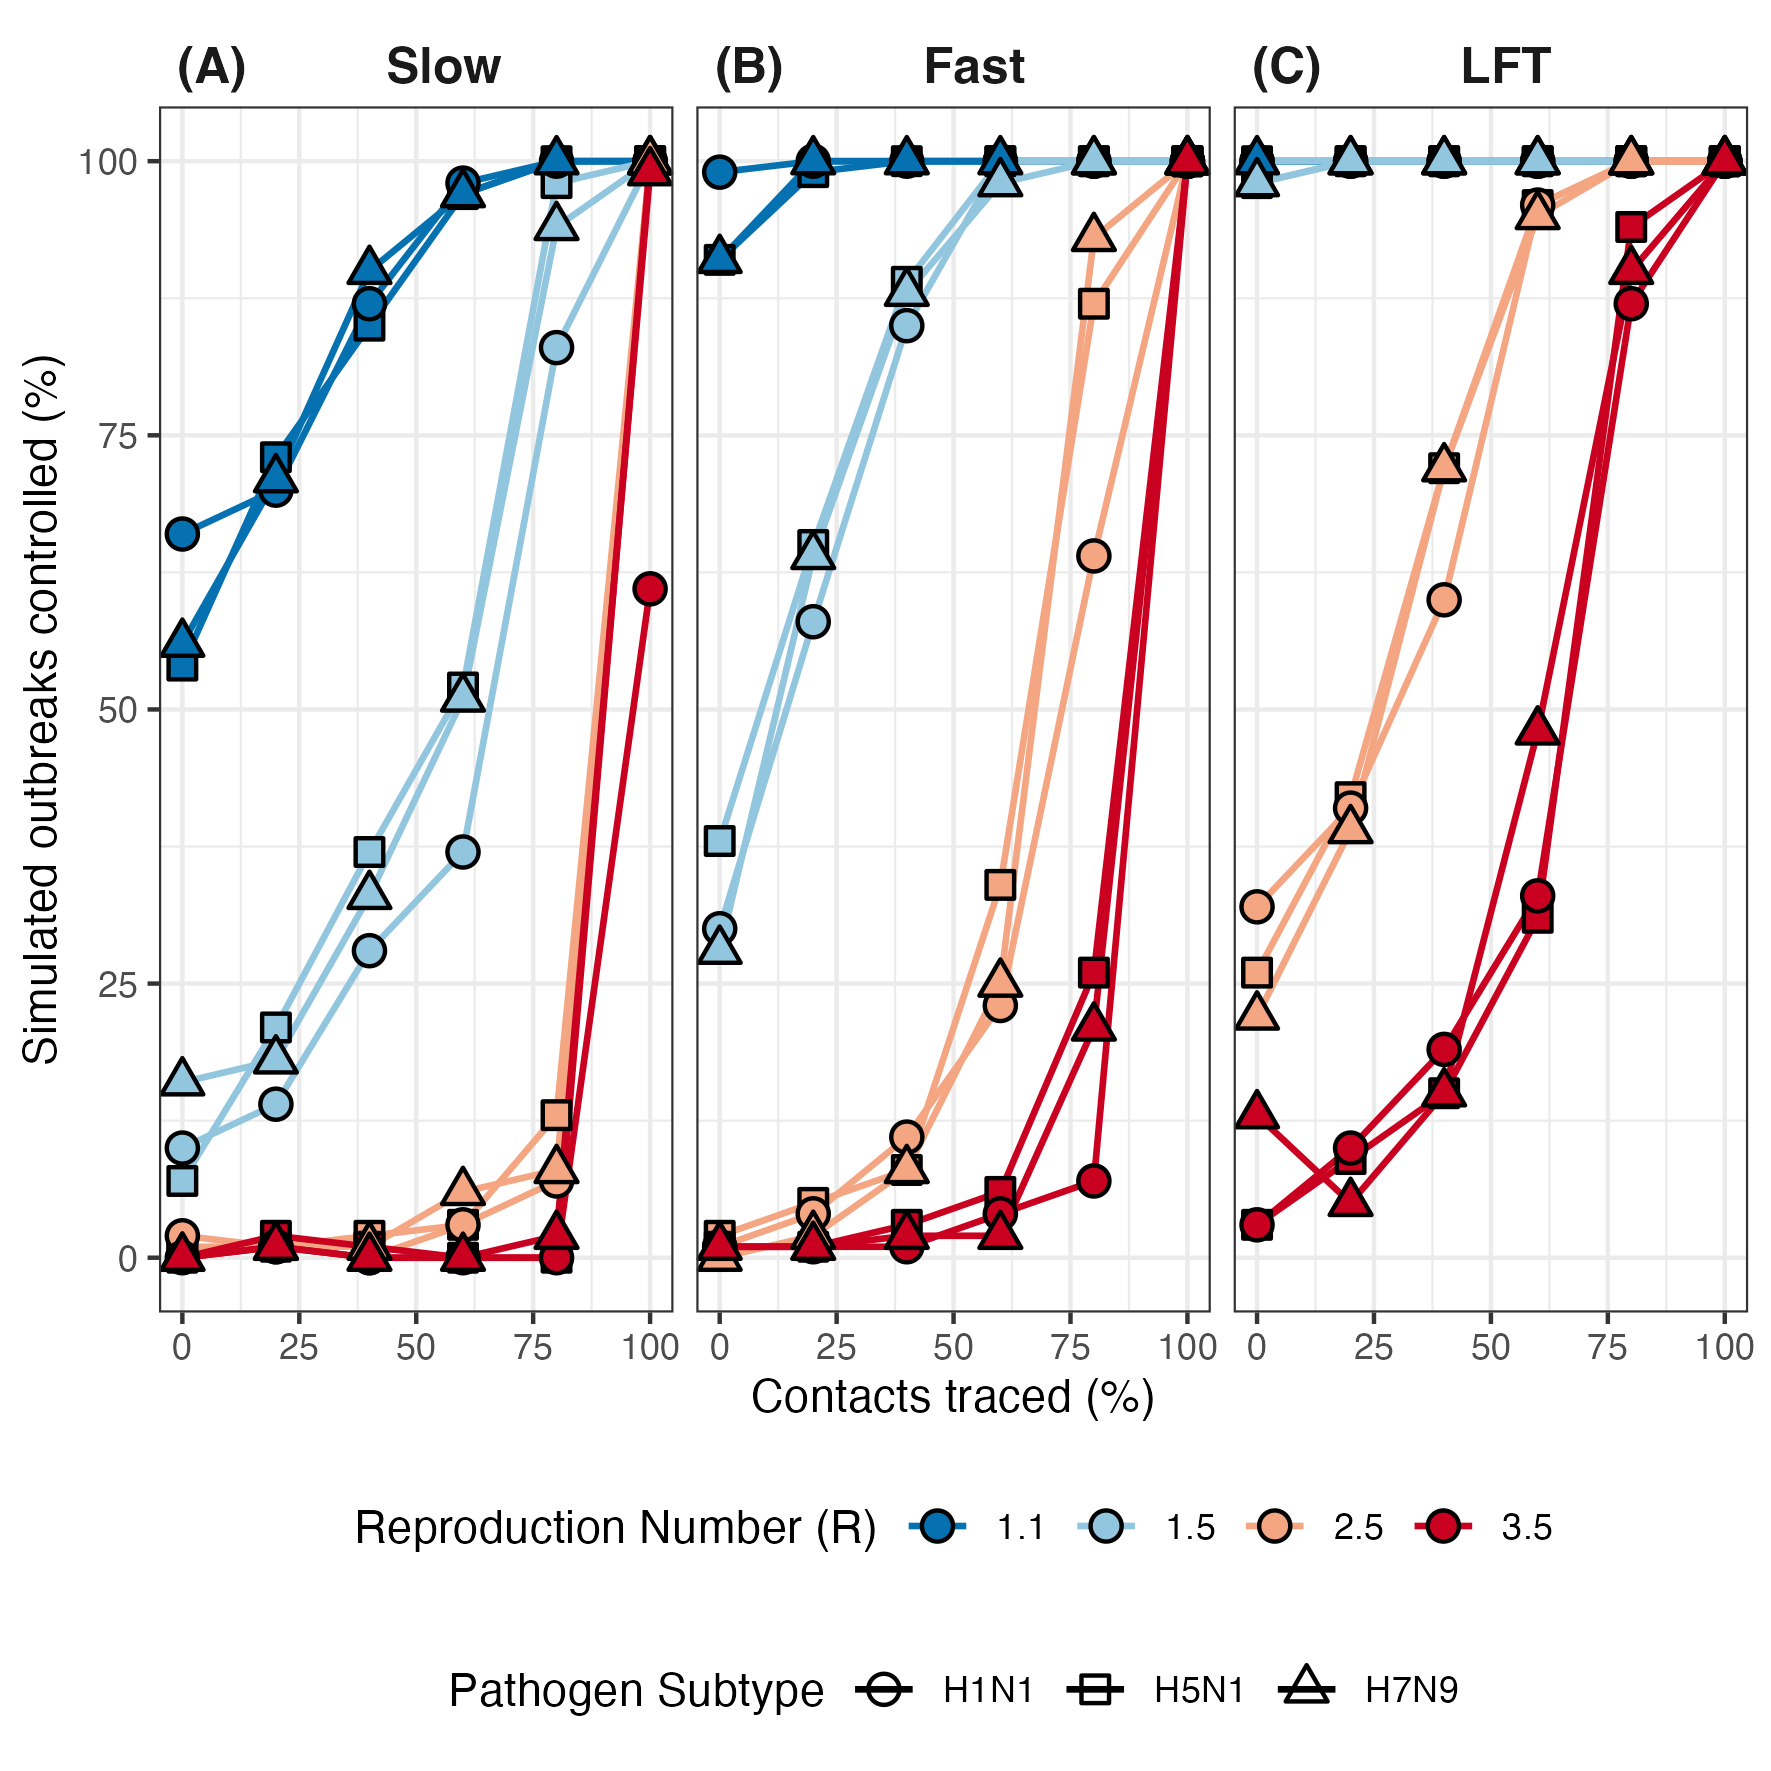
\includegraphics[width=\textwidth]{../plots/prop_outbreak_control_reproduction_number.png}
\caption{The percentage of outbreaks controlled across values of isolation and contact tracing effectiveness, for outbreaks with an assumed reproduction number ($R$) of either 1.1 or 1.5. This is for a baselines scenario where the number of initial cases is 10, the proportion of presymptomatic transmission is 15\%, all cases are assumed symptomatic, and the onset-to-isolation delay is assumed to be SARS-like.}
\label{fig:prop-outbreak-control-R}
\end{figure}

\clearpage

The ability to control an epidemic that can readily transmit human-to-human is moderated by the initial number of infectious individuals that seed the outbreak. The higher the number of cases the less chance that stochastic extinction of a transmission chain will end the whole epidemic. For an influenza pandemic, the number of initial infected individuals influences efficacy of control-by-isolation at all transmissibility scenarios evaluated ($R \in \{1.1, 1.5, 2.5, 3.5\}$, Figure \ref{fig:prop-outbreak-control-num-init-cases}). When $R = 1.1$ most outbreaks can be controlled without isolation and contact tracing, even with 40 initial infectors Figure \ref{fig:prop-outbreak-control-num-init-cases}). When $R = 1.5$ the increase in the number of initial infections from 5 to 20 has a large decrease in outbreaks controlled at low levels of contact tracing, the same pattern when the number of initial infectors is twofold larger at 40, but these differences in outbreak control diminish as contact tracing increases towards 100\% (Figure \ref{fig:prop-outbreak-control-num-init-cases}). When the number of cases seeding the outbreak is $>20$ at $R>2.5$ a large proportion of outbreaks become uncontrollable until contact tracing reaches $>60\%$. In the worst case transmissibility scenario ($R = 3.5$) if contact tracing is not activated until at least 20 individuals are infected then close to 100\% of contacts with need to be traced in order to control the majority of outbreaks (Figure \ref{fig:prop-outbreak-control-num-init-cases}).  \\

\begin{figure}[ht]
\centering
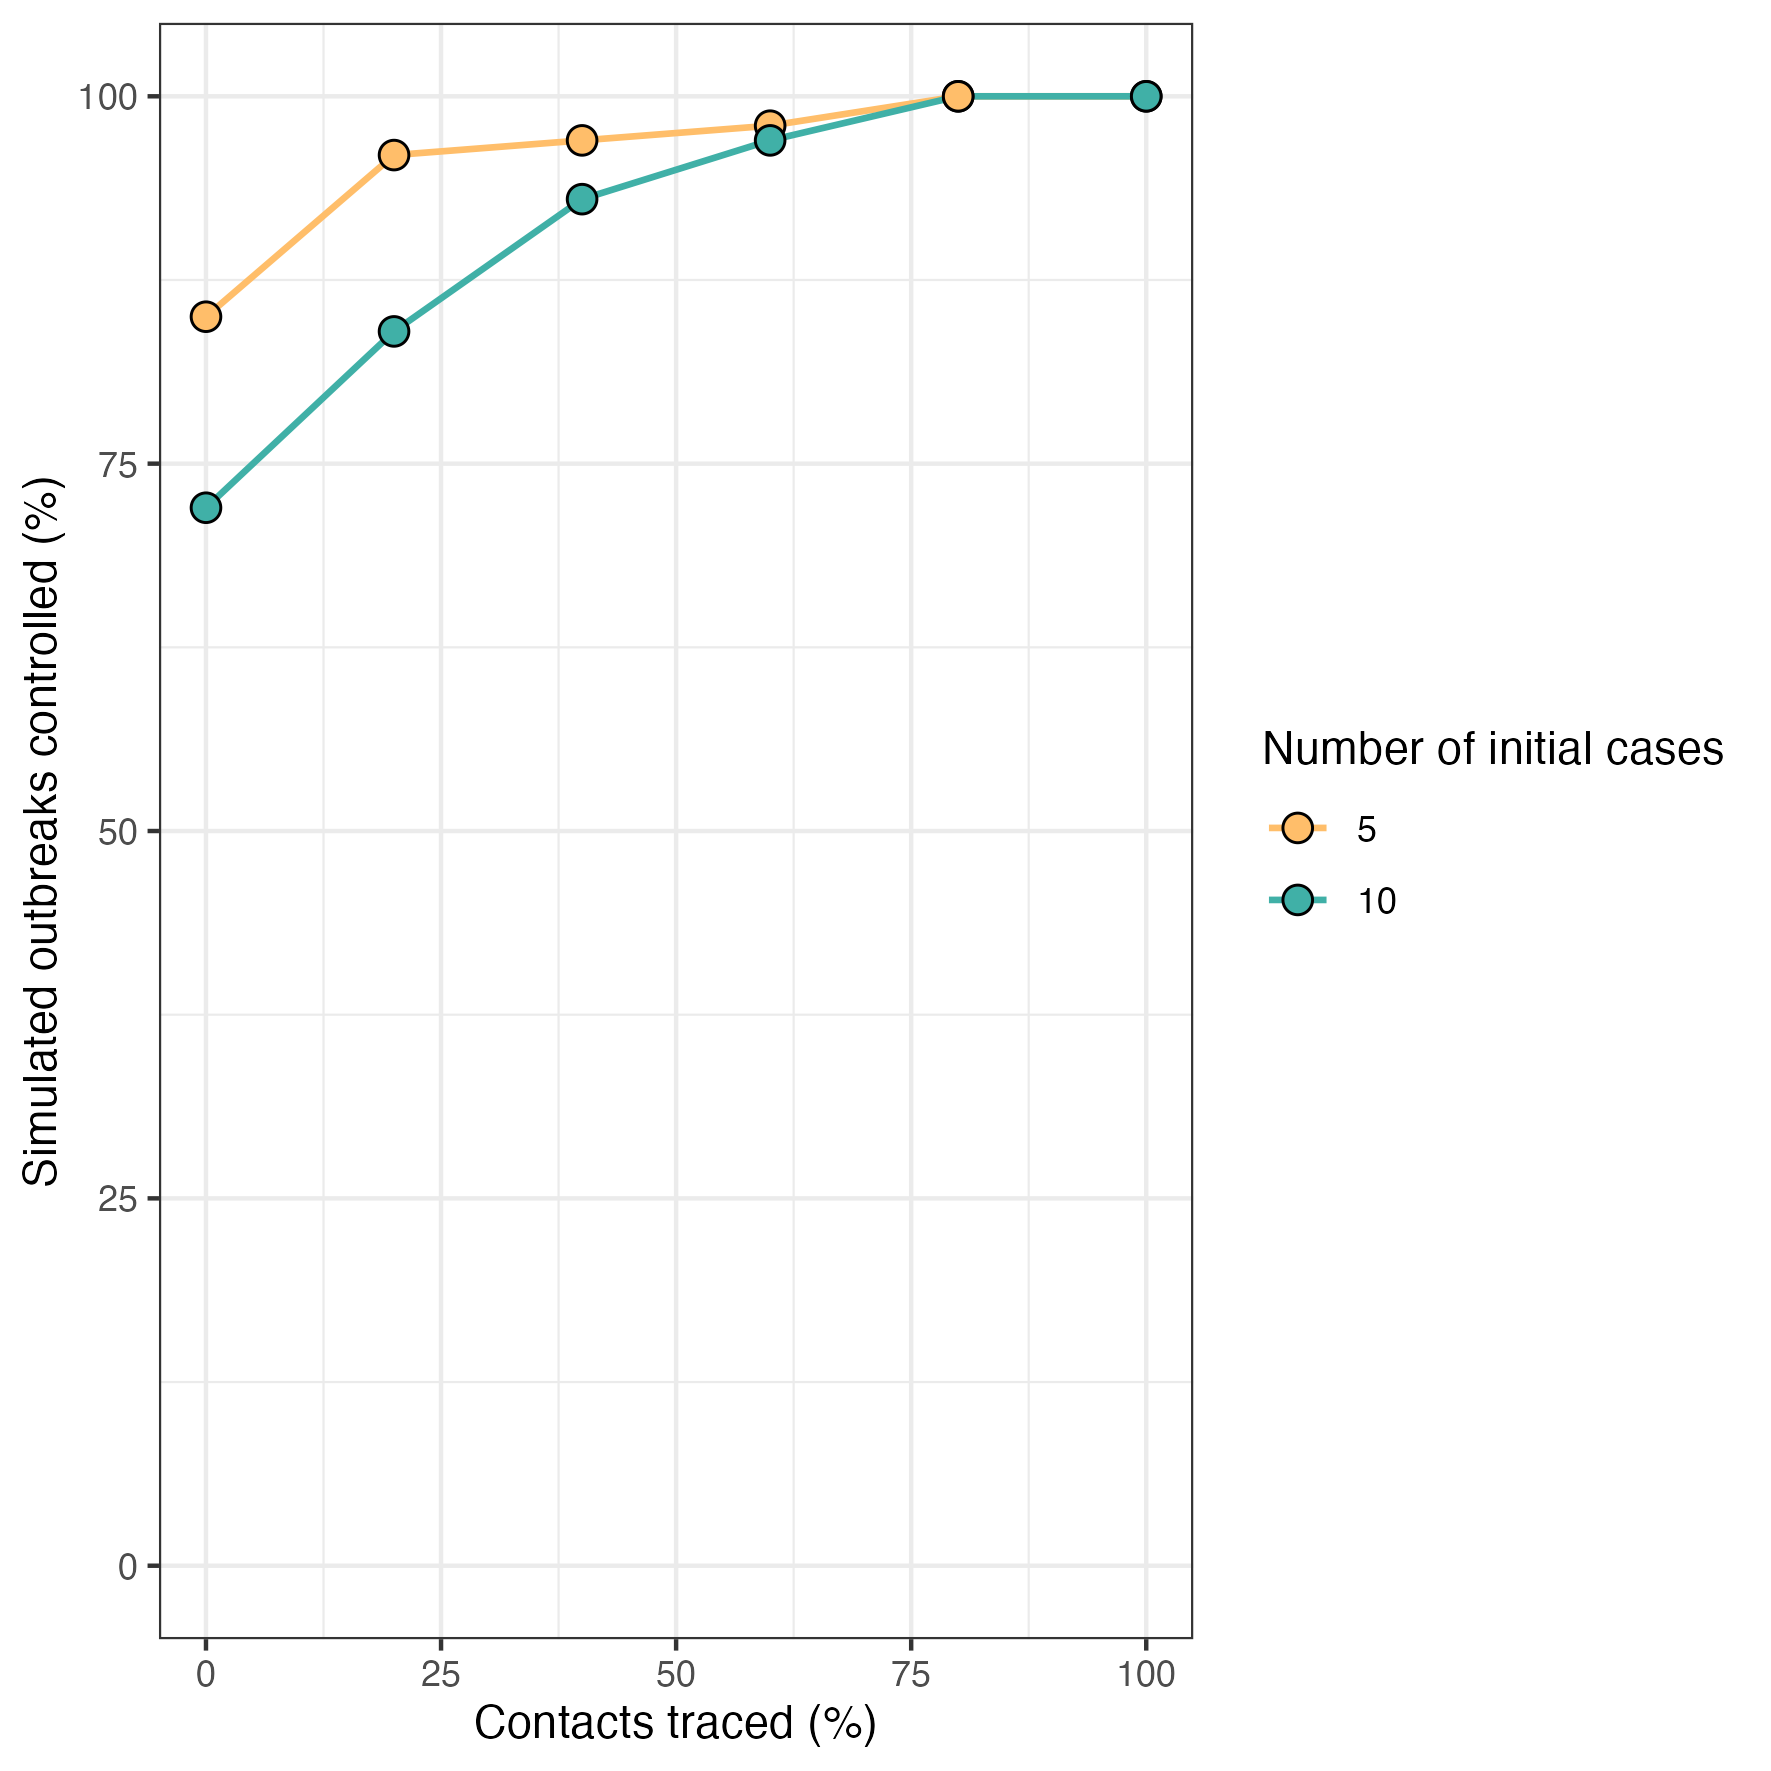
\includegraphics[width=\textwidth]{../plots/prop_outbreak_control_num_init_cases.png}
\caption{The percentage of outbreaks controlled across values of isolation and contact tracing effectiveness, for outbreaks with an initial number of seeding infections assumed to be either 5 or 10. This is for a baselines scenario where the reproduction number is 1.5, the proportion of presymptomatic transmission is 15\%, all cases are assumed symptomatic, and the onset-to-isolation delay is assumed to be SARS-like.}
\label{fig:prop-outbreak-control-num-init-cases}
\end{figure}

\clearpage

\begin{figure}[ht]
\centering
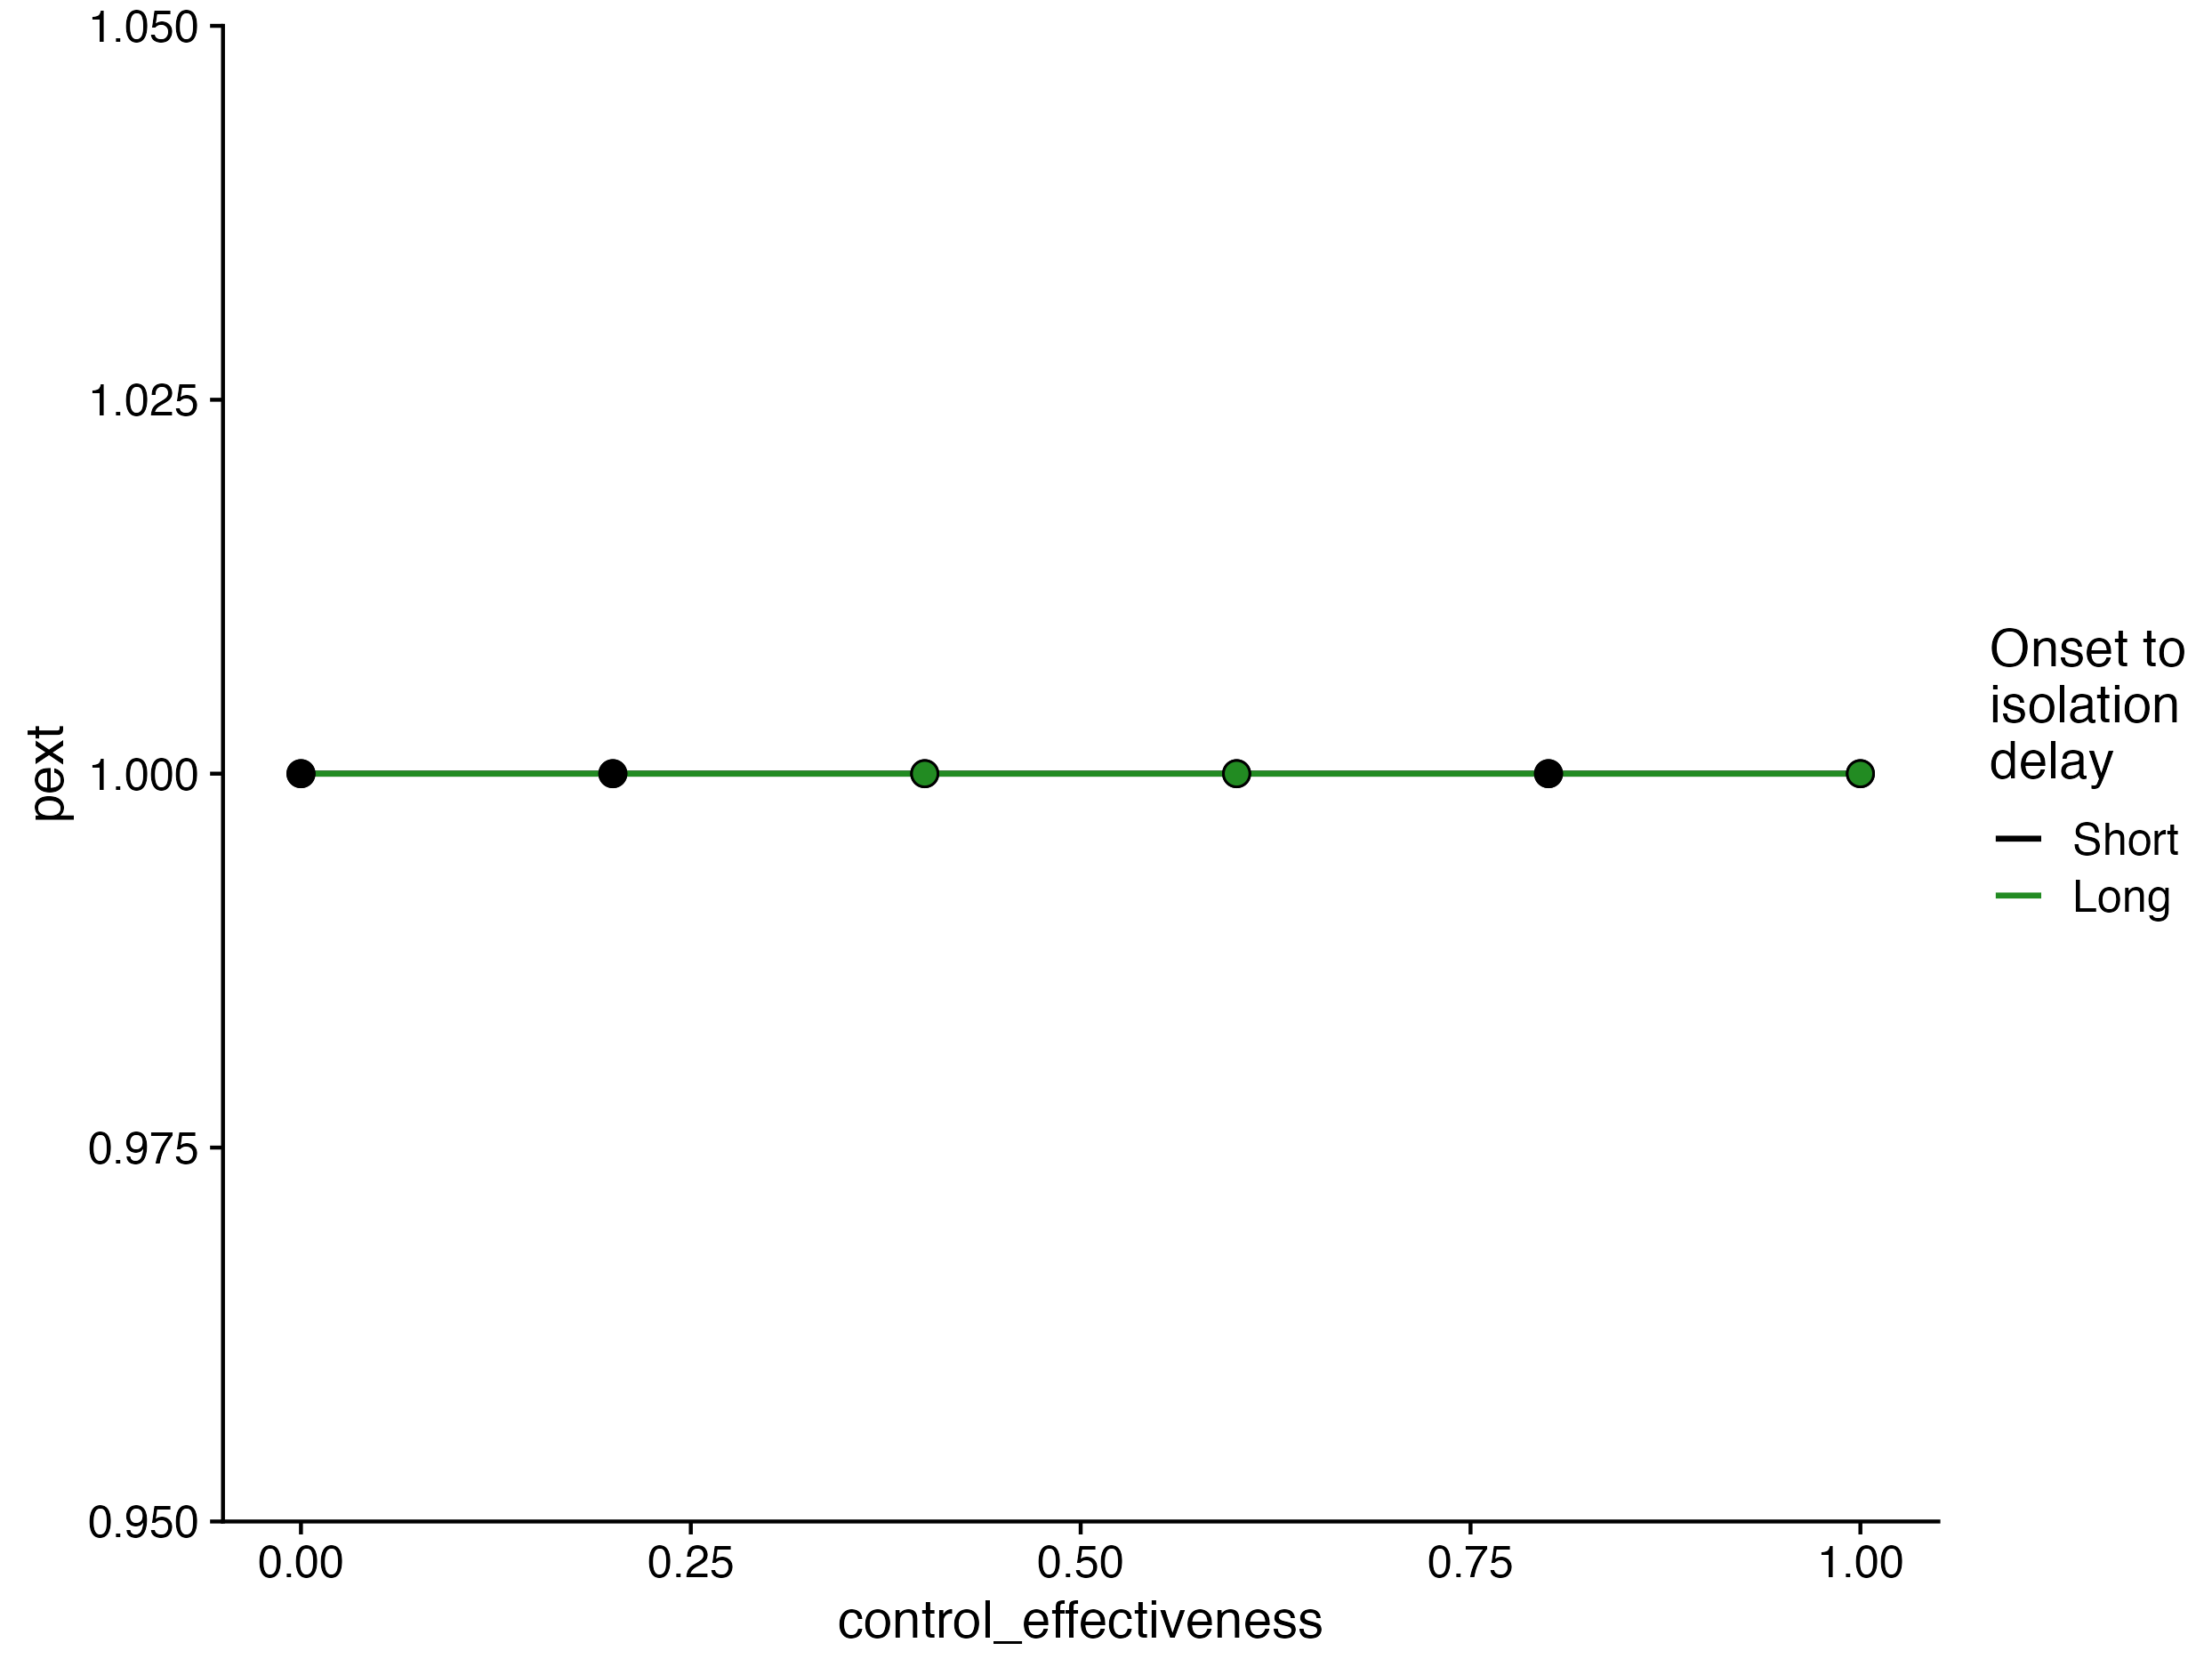
\includegraphics[width=\textwidth]{../plots/prop_outbreak_control_onset_to_isolation.png}
\caption{The percentage of outbreaks controlled across values of isolation and contact tracing effectiveness, for outbreaks with an onset-to-isolation delay distribution that is either SARS-like, or COVID-19-like (from Wuhan). This is for a baselines scenario where the reproduction number is 1.5, the proportion of presymptomatic transmission is 15\%, all cases are assumed symptomatic, and the number of initial infections is 10.}
\label{fig:prop-outbreak-control-onset-to-isolation}
\end{figure}

\section*{Discussion}

\begin{itemize}
\item This study has looked at the feasibility and effectiveness of isolation and contact tracing for influenza subtypes that have cause epidemic outbreaks.
\item Outbreaks controlled at 50\% of contacts traced and isolated is over ??\%, highlighting the effectiveness of this intervention for infectious diseases are not highly transmissible between humans.
\item Discuss the existing flu vaccines and antivirals that can be used an interventions in addition to NPIs
\item In modelling the effectiveness of isolation and contact tracing we have assumed that there is no capacity limits on contact tracing, which does not hold in large outbreaks such as SARS-CoV-2 (ref). We also ignore potential socio-political factors that would prevent health worker from visiting or contacting infected individuals or contacts of infected individuals (Dhillon and Kelly, 2018). We also did not consider zoonotic spillover infections or formite transmission.
\item Digital tracing has capacity for large-scale contact tracing (pingdemic), also rapid tests are a complementary approach for limiting spread.
\item In this study we model isolation and contact tracing as the sole intervention in containing an influenza outbreak. This is to provide an assessment of its effectiveness for rapidly transmission and potentially highly transmissible subtypes. However, in reality, pandemic preparedness to a pandemic potential influenza would not need to deploy interventions, such as contact tracing individually or sequentially, instead they can be used in combination, such as antivirals (e.g. oseltamivir), rapid tests, contact tracing, and vaccination.
\item Antivirals for half the UK, these can be deployed in rapid response to flu pandemic.
\item In this study we have parameterised the transmission model with parameter from avian influenza subtypes (H5N1 and H7N9) and a influenza subtype that caused an epidemic in the recent past (H1N1), and response delays from SARS and COVID-19 outbreaks. However, these results can be used to inform other influenza subtypes that exhibit similar epidemiological characteristics in transmissibility and severity from past outbreaks (H2N2 and H3N2) and still exist in animal reservoirs for potential spillovers back into human populations (ref).
\item This study used a branching process model to simulate individual-level transmission and intervention. The model assumes an infinite population size with no interdependence of isolation and contact tracing between cases whereby a case may be in contact with multiple infectors and only needs to be traced in time by one contact to prevent transmission, as could happened in a fixed random network transmission model. It is unlikely that this model structure difference would have a considerable different on our results for the control of disease outbreaks with contact tracing. We suppose that because our model requires isolation sampled for a single individual, our results are more conservative on the ability to control outbreaks, and that using a random network model would indicate an increased effectivness of contact tracing (Juul and Strogatz, 2023). The infinite population assumption also means that although isolated individuals are assumed to not transmit, there are always other individuals that non-isolated infectors can transmit to, whereas a fixed random network model that assumes optimal indefinite isolation will block of parts of the network and overestimate contact tracing effectiveness (Juul and Strogatz, 2023).
\item The reproduction number for H5N1 (including clade 2.3.4.4b) and H7N9 influenza subtypes have been estimated to be far below 1 (Ward et al., Garg et al., 2025). Therefore, the transmissibility scenarios explored in this study are speculative and assume that pathogen evolution increases human-to-human transmission potential. If transmissibility of these avian influenza subtypes remains constant over time then outbreaks are expected to be subcritical and will not produce epidemics and thus not require interventions. If cases of avian influenza are detected with routine surveillance without a known animal source, it may indicate sustained human-to-human transmission and can be a trigger to commence isolation and contact tracing while the number of initial cases is presumed small, which as we show increases epidemic controllability (Figure \ref{fig:prop-outbreak-control-num-init-cases}).
\item This study has evaluated the ability to control the outbreak of an infectious disease independent on its severity. Infection severity and fatality risks are of course critical when formulating a pandemic response plan. By understanding the efficacy of isolation and contact trace for a given epidemiological characterstic, outbreak mortality and morbidity can hopefully be minimised by reducing disease incidence over time to elimination.
\item Our branching process model used a simple forward contact-tracing mechanism that reduces the number of secondary contacts based on the timing of isolation of symptomatic cases. This contact tracing stragety is minimal cost and effort. In scenarios where outbreaks are uncontrolled a more comprehensive and costly contact tracing system where infectors and contacts of infectors (i.e. backward and forward contact tracing) are followed up, which has been shown to be more effective at outbreak containment (Klinkenberg et al., 2006).
\item Isolation and contact tracing complementing in combination with other quickly available measures for pandemic potential influenza strains, such as rapid testing and antivirals \citep{haydenPerspectivesAntiviralUse2001}.
\end{itemize}

\bibliographystyle{plainnat}
\bibliography{FluTracer.bib}

\clearpage

\section*{Supplementary Material}

\setcounter{figure}{0}
\renewcommand{\thefigure}{S\arabic{figure}}


\begin{figure}[ht]
\centering
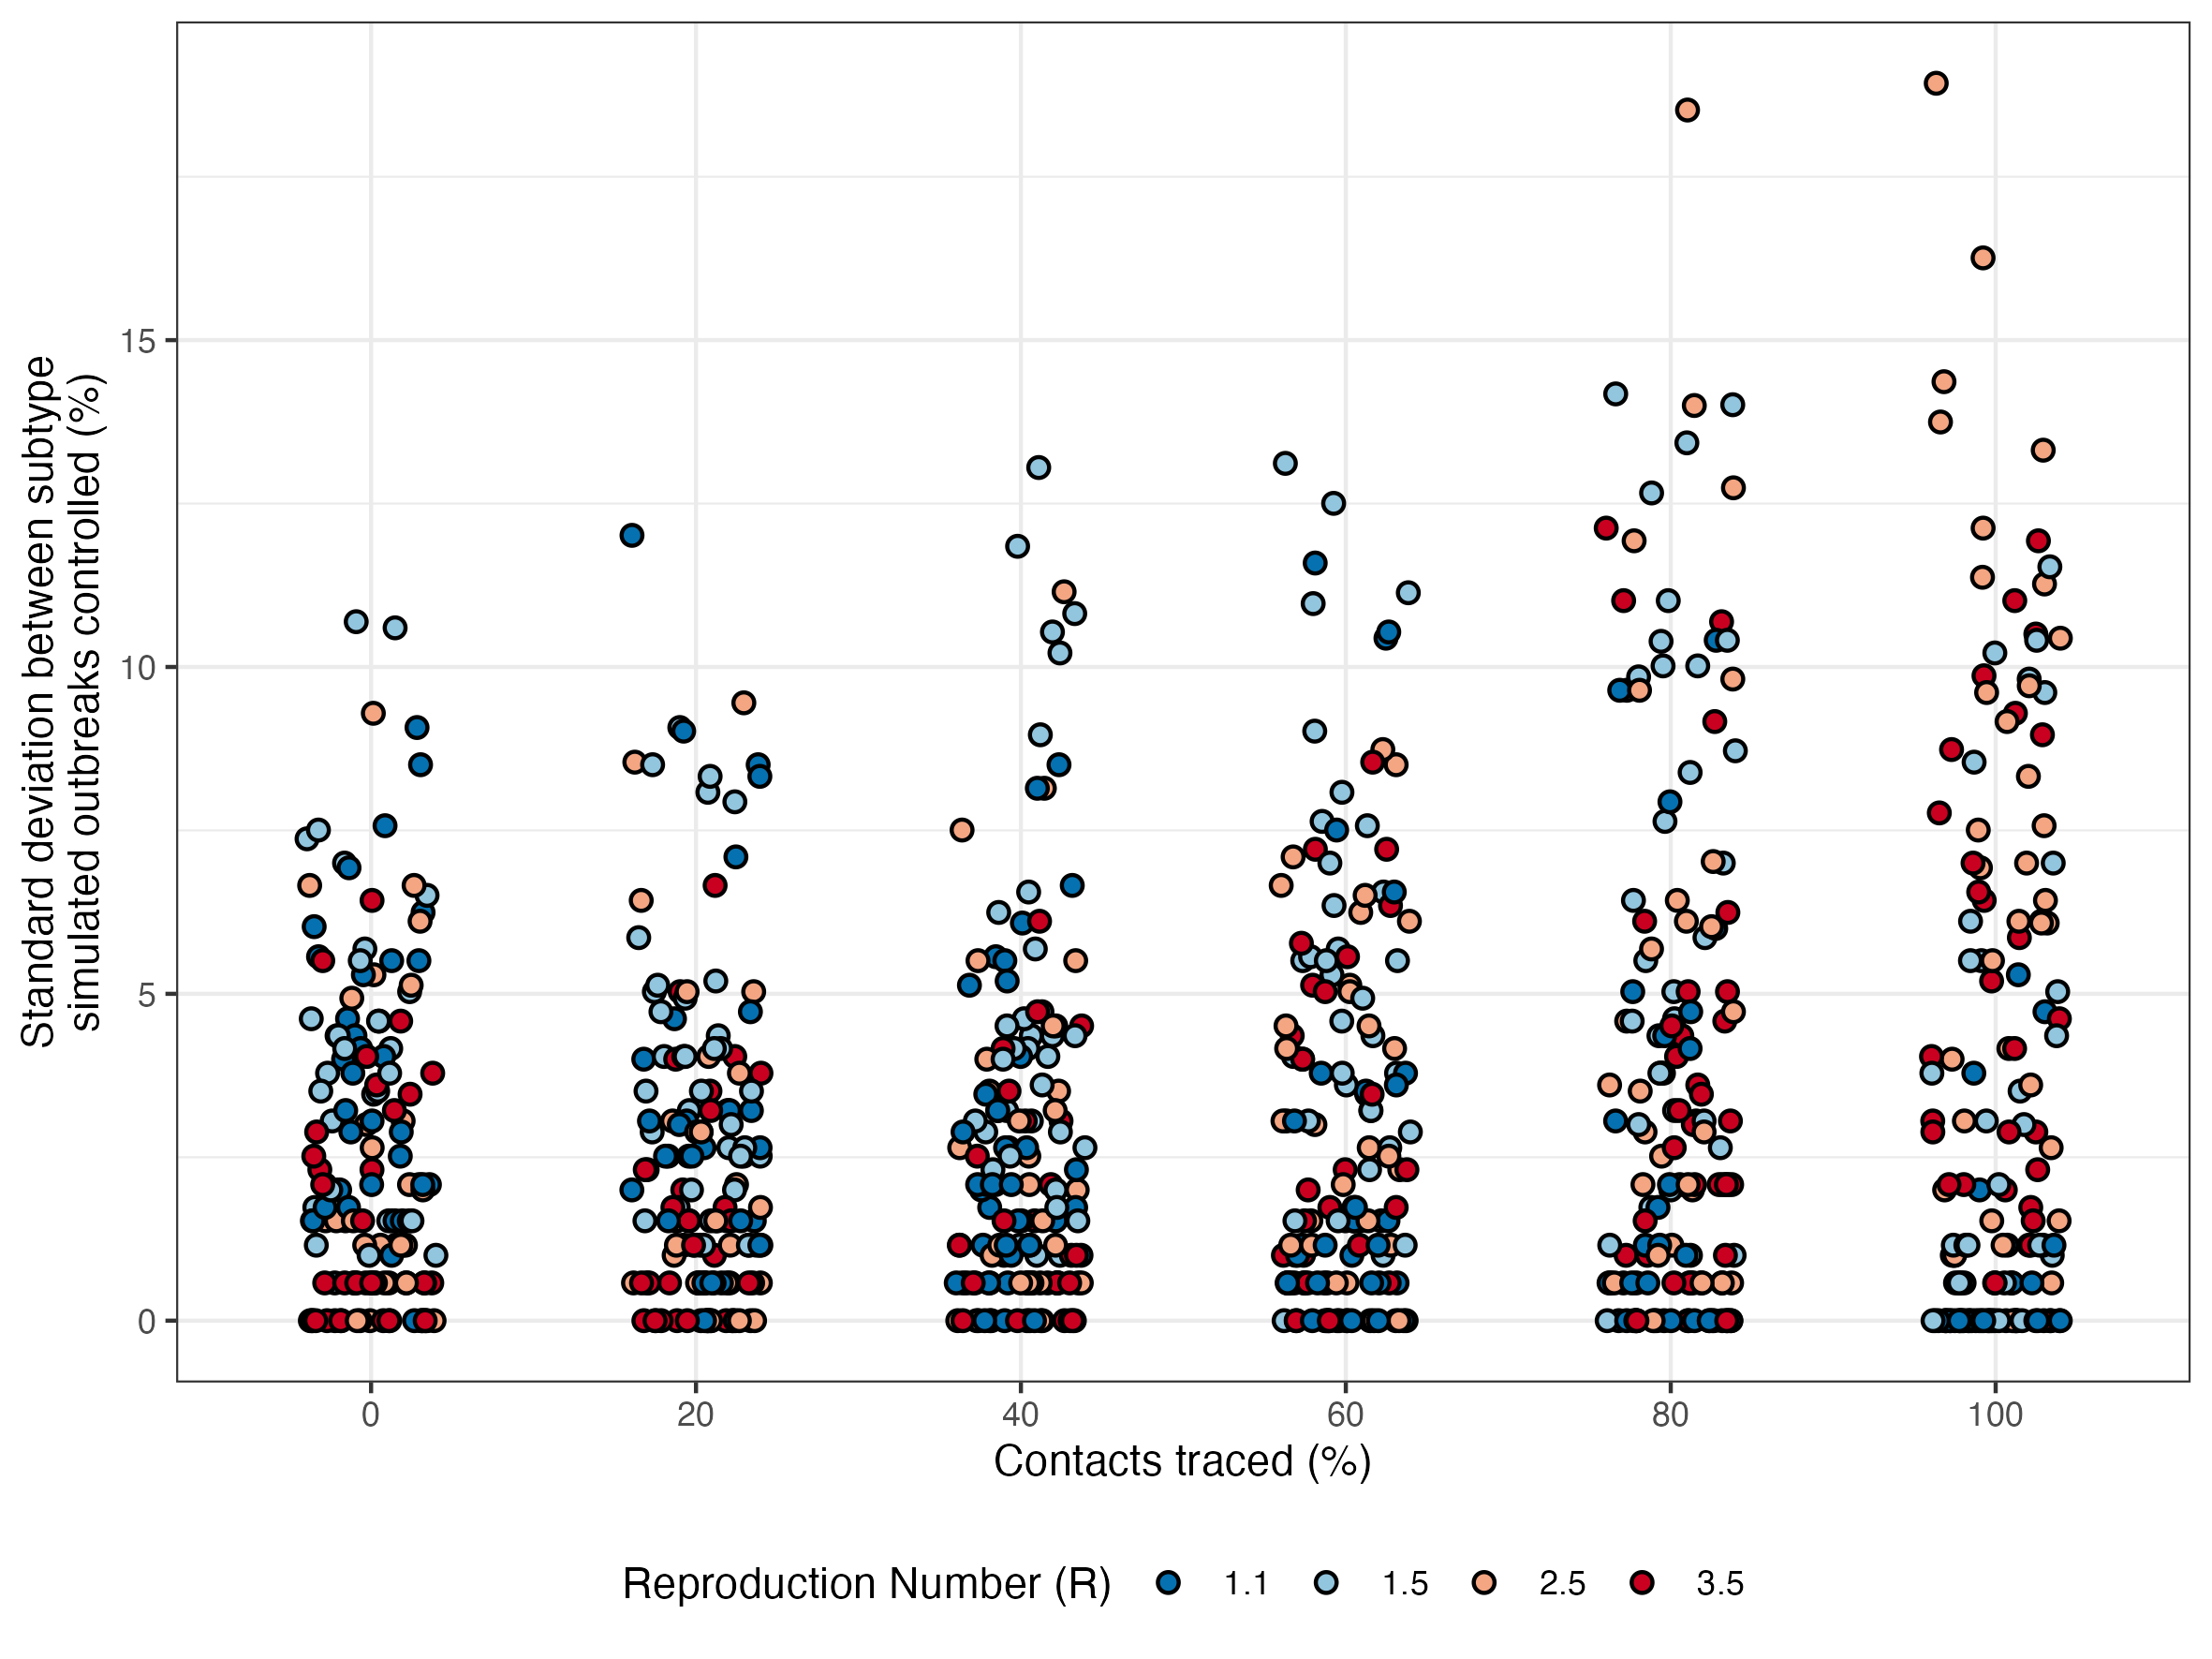
\includegraphics[width=\textwidth]{../plots/prop_outbreak_control_var_reproduction_number.png}
\caption{The standard deviation of the percentage of outbreaks controlled between influenza subtypes (H1N1, H5N1, H7N9), across percentages of contacts traced. Points are jittered horizontally reduce overlap.}
\label{fig:prop-outbreak-control-var-R}
\end{figure}

\end{document}
